\documentclass{ipn}

\usepackage{ipnstyle}
\usepackage{lipsum}
\usepackage{graphicx}
\usepackage{float}
\usepackage{caption}
\usepackage{subcaption}
\usepackage{bookmark}
\usepackage{hyperref}
\usepackage{minted}
% \usepackage{cite}

\author{Lic. Your Name}
\title{Your awsome thesis title}
\schoolname{Centro de Investigación en Computación}
\degree{Maestría en Ciencias de la Computación}
\advisor{Dr. Main Advisor}
\coadvisor{Dr. Co Advisor}
\academicyear{Enero 2025}

\hypersetup{
    colorlinks=false,
    pdfauthor={Your Name},
    pdftitle={Your awsome thesis title},
    pdfsubject={Thesis},
    pdfkeywords={keyword1, keyword2, keyword3}
    pdfproducer={Latex with hyperref},
    pdfcreator={pdflatex}
}

\addbibresource{./references.bib}
\pagestyle{headings}

\begin{document}
\frontmatter
    \maketitle
    \input{frontmatter/advertisement}
    \chapter{Resumen}
\lipsum[1-3]

\chapter{Abstract}
\lipsum[1-3]
    \chapter{Acknowledgments}
\lipsum[1]
    \tableofcontents
    \listoffigures
    \listoftables
    \listofalgorithms

\mainmatter
    \chapter{Introduction}\label{ch:Introduction}
\lipsum[1]

\section{Research problem}
\lipsum[1]
\begin{definition}[Open space]
A subset $U$ of a metric space $(M, d)$ is called open if, for any point $x$ in $U$, there exists a real number $\epsilon > 0$ such that any point $y\in M$ satisfying $d(x, y) < \epsilon$ belongs to $U$. Equivalently, $U$ is open if every point in $U$ has a neighborhood contained in $U$.
\end{definition}
\lipsum[1]

\section{Objectives}
\subsection{General objective}
Lorem ipsum dolor sit amet, consectetuer adipiscing elit~\cite{adam2015higgs, atlas2014neural, baldi2014searching}. Ut purus elit, vestibulum ut, placerat ac, adipiscing vitae, felis. Curabitur dictum gravida mauris. Nam arcu libero, nonummy eget, consectetuer id, vulputate a, magna.

\subsection{Specific objectives}
Lorem ipsum dolor sit amet, consectetuer adipiscing elit:
\begin{itemize}
    \item Lorem ipsum dolor sit amet, consectetuer adipiscing elit. Ut purus elit, vestibulum ut, placerat ac, adipiscing vitae, felis. Curabitur dictum gravida mauris.
    \item Nam arcu libero, nonummy eget, consectetuer id, vulputate a, magna.
    \item  Pellentesque habitant morbi tristique senectus et netuset malesuada fames ac turpis egesta
\end{itemize}

\section{Justification}
\lipsum[1]

\section{Project scope and limitations}
\lipsum[1]
\begin{theorem}
The kernel of a linear transformation from a vector space V to a vector space W is a subspace of V.
\end{theorem}
\begin{proof}
    Suppose that u and v are vectors in the kernel of L.  Then 
    \begin{equation}
        L(u) = L(v) = 0
    \end{equation}
    We have
    \begin{equation}
        L(u + v) = L(u) + (v) = 0 + 0 = 0 
    \end{equation}
    and
    \begin{equation}
        L(cu) = cL(u) = c0 = 0
    \end{equation}
    Hence $u + v$ and cu are in the kernel of $L$. We can conclude that the kernel of $L$ is a subspace of $V$.
\end{proof}
\lipsum[1]

\begin{algorithm}[H]
    \caption{Descenso de gradiente estocástico}\label{alg:SGD}
    \hspace*{\algorithmicindent} \textbf{parameters} \\
    \hspace*{\algorithmicindent}\hspace*{\algorithmicindent} Número de iteraciones $\tau$ \\
    \hspace*{\algorithmicindent}\hspace*{\algorithmicindent} Tasa de aprendizaje $\eta$ \\
    \hspace*{\algorithmicindent}\hspace*{\algorithmicindent} Parámetro de regularización $\lambda$ \\
    \hspace*{\algorithmicindent} \textbf{input} \\
    \hspace*{\algorithmicindent}\hspace*{\algorithmicindent} Pesos iniciales $\mathbf{w}^{(1)}$ \\
    \hspace*{\algorithmicindent}\hspace*{\algorithmicindent} Gradiente en una muestra $\mathcal{Q}_i(w)$
    \begin{algorithmic}[1]
        \Procedure{SGD}{$\mathbf{w}^{(1)}, \sigma$}
        \For{$i \gets 1, 2, \dots, \tau$}
        \State Selecciona una muestra $(\mathbf{x}, \mathbf{y})\sim D$
        \State Calcula el gradiente $\nabla\mathcal{Q}_i(w)$ para la muestra $(\mathbf{x}, \mathbf{y})$
        \State Asigna $\mathbf{w}^{(i+1)} \gets \mathbf{w}^{(i)} - \eta(\nabla\mathcal{Q}_i(w) + \lambda\mathbf{w}^{(i)})$
        \EndFor
        \EndProcedure
    \end{algorithmic}
\end{algorithm}

\section{Hypothesis}
\lipsum[1-2]

\section{Project organization}
\lipsum[1-2]
    \chapter{Conclusions}\label{ch:Conclusions}
\lipsum[1]
\begin{table}[hbtp]
    \centering
    \begin{tabular}{@{}*{2}{p{0.5\textwidth}}@{}}
        \toprule
        \textbf{Correct} &  \textbf{Incorrect}
        \\
        \midrule
        \enquote{This is an \enquote{inner quote} inside an outer quote}
        &
        "This is an 'inner quote' inside an outer quote"
        \\
        \bottomrule
    \end{tabular}
    \caption[Quotation marks]
    {Proper quotation mark usage.
    The \texttt{\textbackslash enquote} command chooses the correct
    quotation marks for the specified language.}
\end{table}
\lipsum[1]

\section{Recommendations and future work}
\lipsum[1]

    \appendix
        \chapter{Simulator}\label{app:Simulator}
\lipsum[1]
\begin{listing}[H]
\begin{minted}[linenos, breaklines]{python}
import torch
import torch.nn as nn
import torch.nn.functional as F

class Net(nn.Module):
    def __init__(self):
        super(Net, self).__init__()
        self.conv1 = nn.Conv2d(1, 6, 5)
        self.conv2 = nn.Conv2d(6, 16, 5)
        self.fc1 = nn.Linear(16 * 5 * 5, 120)  # 5*5 from image dimension
        self.fc2 = nn.Linear(120, 84)
        self.fc3 = nn.Linear(84, 10)
    def forward(self, x):
        # ...
        return x

net = Net()
print(net)
\end{minted}
\caption{A basic neural network.}
\end{listing}
\lipsum[1]
        \chapter{Proof of theorem}\label{app:Proof of theorem}
\lipsum[1]
\begin{figure}[thbp]
    \centering
    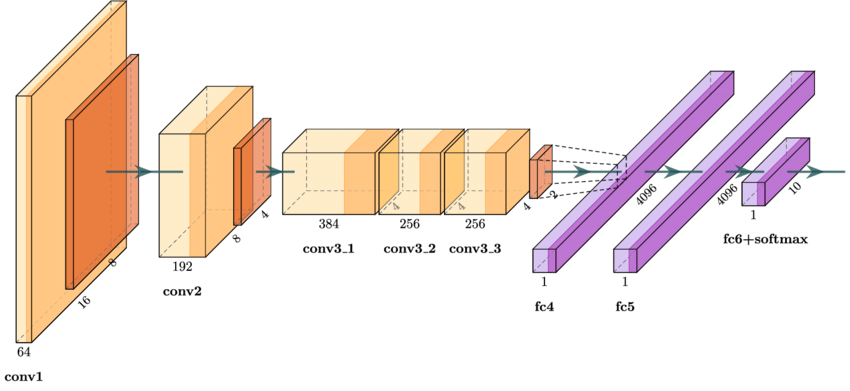
\includegraphics[width=\textwidth]{img/appendixA/alexnet.png}
    \caption{AlexNet architecture.}\label{fig:alexnet}
\end{figure}
\lipsum[1]
\begin{align}
     \vec{\nabla} \cdot \vec{E} \quad &=\quad\frac{\rho}{\epsilon_0} &&\text{Gauss's Law} \\      
    \vec{\nabla} \cdot \vec{B} \quad &=\quad 0 &&\text{Gauss's Law for Magnetism}\\
    \vec{\nabla} \times \vec{E} \quad &=\hspace{10pt}-\frac{\partial{\vec{B}}}{\partial{t}} &&\text{Faraday's Law of Induction} \\ 
    \vec{\nabla} \times \vec{B} \quad &=\quad \mu_0\left( \epsilon_0\frac{\partial{\vec{E}}}{\partial{t}}+\vec{J}\right) &&\text{Ampere's Circuital Law}
\end{align}

We can find more information in~\cite{li2018deep}.

\backmatter
    \bookmarksetup{startatroot}
    \printbibliography[heading=bibintoc]
\end{document}